1) Convertir la coordenada ${\left(1,2,2\right)}$ rectangular al sistema esférico.
\[\rho = \sqrt{x^{2}+y^{2}+z^{2}} = \sqrt{1^{2}+2^{2}+2^{2}} = 3\]
\[\varphi = \arccos\left(\frac{z}{p}\right) = \arccos\left(\frac{2}{3}\right) = 48.19^{\circ} = 0.84\]
\[\theta = \arctan\left(2\right) = 63.43^{\circ} = 1.11\]

\vspace{4mm}
2) Convertir la coordenada ${\left(-2,2\sqrt{3},4\right)}$ rectangular al sistema esférico.
\[\rho = \sqrt{x^{2}+y^{2}+z^{2}} = \sqrt{(-2)^2+(2\sqrt{3})^{2}+4^{2}} = 4 \sqrt{2}\]
\[\varphi = \arccos\left(\frac{4}{4\sqrt{2}}\right) = 45^{\circ} = \frac{\pi}{4}\]

\vspace{4mm}
Es importante analizar las coordenadas ${\left(x,y\right)}$, es decir ${\left(-2,2\sqrt{3}\right)}$ para determinar su cuadrante y de esa manera saber cómo proceder en el proceso de obtención del valor de ${\theta}$. Como en éste caso, se encuentra en el segundo cuadrante, entonces no es útil el uso de la ecuación deducida anteriormente para encontrar ${\theta}$, sino determinar el ángulo complementario ${\alpha}$ y luego realizar la resta de dicho ángulo para determinar ${\theta}$, se puede visualizar en la siguiente imagen.

\begin{figure}[H]
  \centering
  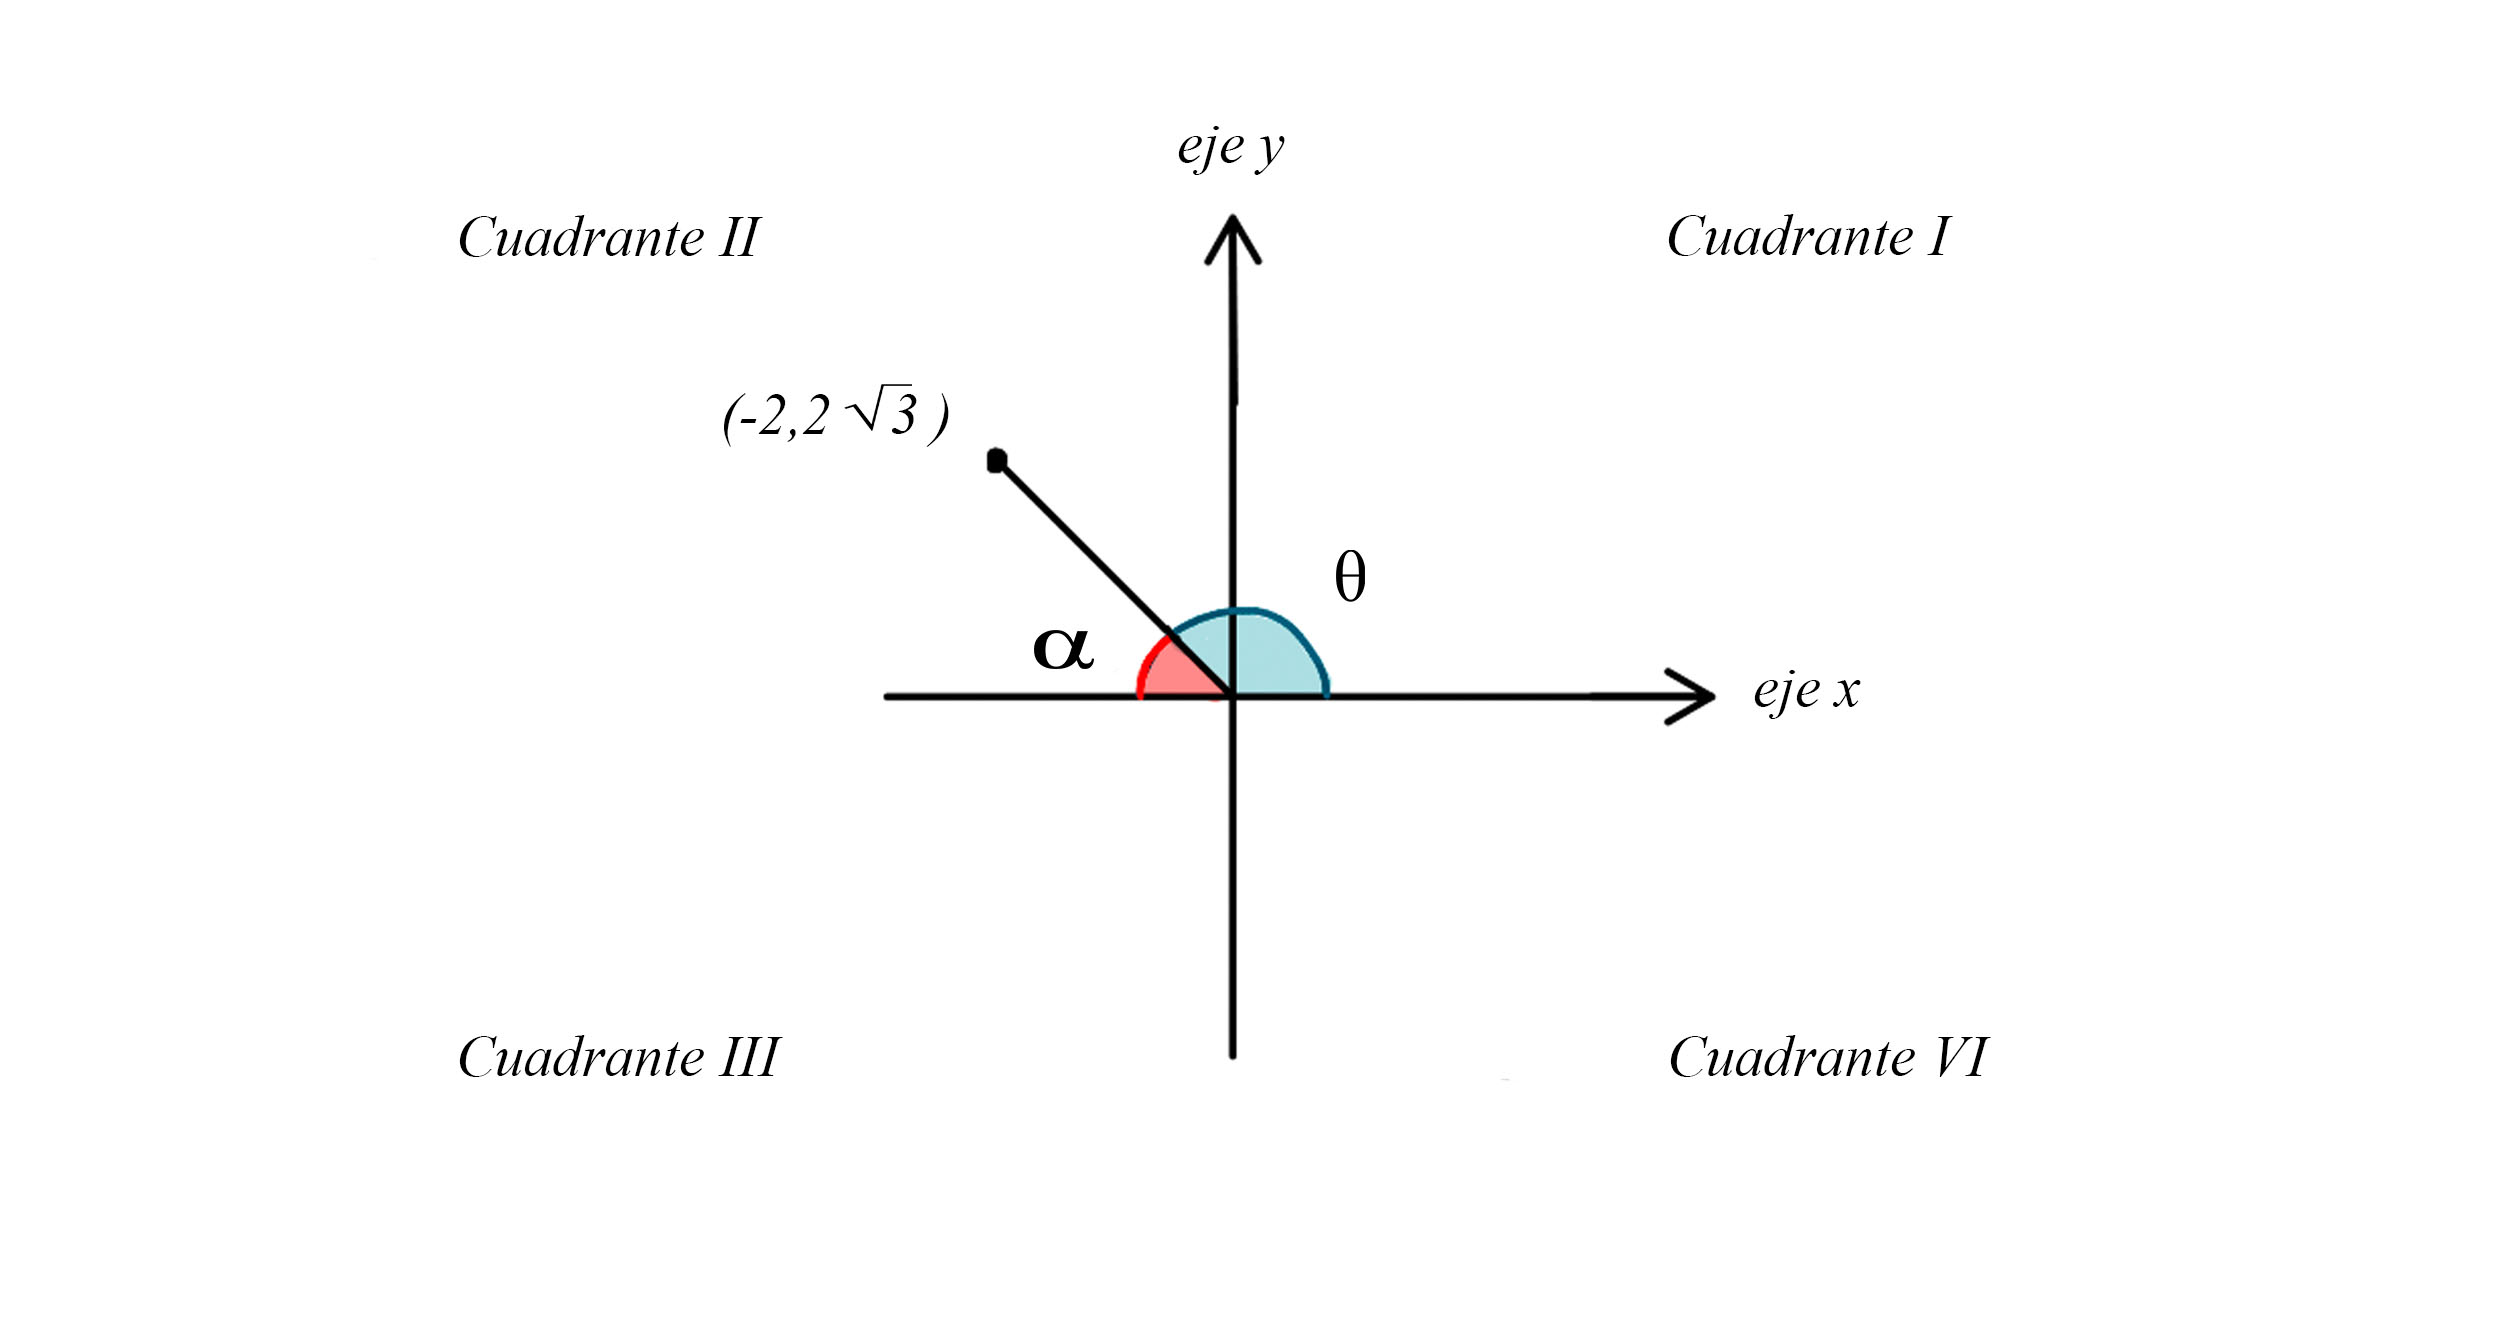
\includegraphics[width=11.17cm, height=5.67cm]{img/graph/segundo_cuadrante.jpg}
  \caption{Punto con coordenadas ${(-2,2\sqrt{3})}$.}
\end{figure}

Donde ${\alpha}$ representa el ángulo de interés para abordar su complemento ${\theta}$. Entonces, para encontrar el ángulo ${\alpha}$ se sabe que:
\[\alpha = \arctan\left(\frac{y}{x}\right) = \arctan \left( \left|\frac{2\sqrt{3}}{-2} \right| \right) = \arctan(\sqrt{3}) = 60^{\circ} = \frac{\pi}{3} \]
\[\therefore \theta = 180^{\circ} - \alpha = 120^{\circ} =\frac{2\pi}{3}\]

\vspace{4mm}
3) Convertir la coordenada ${\left(-\sqrt{3},-1,-2\sqrt{3}\right)}$ a su forma esférica.
\[\rho = \sqrt{x^{2}+y^{2}+z^{2}} = \sqrt{\left(-\sqrt{3})^{2}+(-1)^{2}+(-2\sqrt{3}\right)^{2}} = 4\]
\[\varphi = \arccos\left(\frac{z}{p}\right) = \arccos\left(\frac{-2\sqrt{3}}{4}\right) = 150^{\circ} = \frac{5\pi}{6} \]

\vspace{4mm}
Nuevamente, primero calculamos el ángulo auxiliar ${\alpha}$ más cercano al eje x de las coordenadas ${\left(x,y\right) = \left(-\sqrt{3},-1\right)}$, como el punto se encuentra en el tercer cuadrante, entonces podremos realizar la suma del valor de ${\alpha}$ a ${180^{\circ}}$ para encontrar el valor de ${\theta}$.
\[\alpha = \arctan\left(\frac{y}{x}\right) = \arctan\left( \left|\frac{-1}{-\sqrt{3}}\right| \right) = 30^{\circ}\]
\[\therefore \theta = 180^{\circ} + \alpha = 210^{\circ} = \frac{7\pi}{6}\]

\cite{lehmann}
